\chapter{Reconstruction and identification of physical objects}
\label{ch:objects}
\epigraph{\emph{“Champions keep playing until they get it right.”}}{Billie Jean King}


The particles (and products of their decays) produced at every collission, interact with the detector in a particular manner according to their nature. The information recollected by all the sub-detectors described in the previous chapter allow for the reconstruction and identification of the physical objects present in each accepted event by the trigger system. Two types of reconstruction and identification exist. The \textit{online} one, is carried out at the same time the \pp collissions take place, and the \textit{offline} one, done after the events are saved to storage. The reconstruction is done event by event, and is carried in the same way for events recorded by the \ac{ATLAS} detector and for simulated \ac{MC} events. In the following, a brief overview of the offline reconstruction and identification of the objects used in this thesis is given.



\fixme{update chapter, see version in spanish}



\section{Track and vertex reconstrucion}

In a high-pile-up event, there can be of the order of 1000 charged particles passing through the \ac{ATLAS} detector. The information from the \ac{ID} (\Sect{\ref{subsec:atlas:atlas:id}}) is used to reconstruct the trajectories of charged particles, called \textit{tracks}.

Tracking charged particles is a critical step in reconstruction. Tracks encode charged particles' momentum and trajectory, playing an essential role in particle identification and primary vertex reconstruction. As the inner detector is closest to the beamline and comprises minimally ionizing detector material with high granularity, it plays the main role in track reconstruction. A charged particle passing through different layers of \ac{ID} leaves a signal via ionization. As the \ac{ID} solenoidal field is homogenous, the resulting trajectory is circular in the \(xy\) plane. Five parameters shown in \Fig{\ref{fig:objects:track_vtx:track_parameters}} define charged particle tracks:
\begin{itemize}
    \item \(q/\pt\): the ratio of the charge and transverse momentum defining the curvature
    \item \(d_0\): the distance of the closest approach to the primary vertex in \(xy\)-plane defining the transverse impact parameter
    \item \(z_0\): the longitudinal impact parameter along the \(z\)-axis
    \item \(\phi_0\): the azimuthal angle
    \item \(\theta_0\): the polar angle of the particle direction oat the closest point of approach~\cite{ATLAS-Tracks-Performance-Run2}.
\end{itemize}

\begin{figure}[ht!]
    \centering
    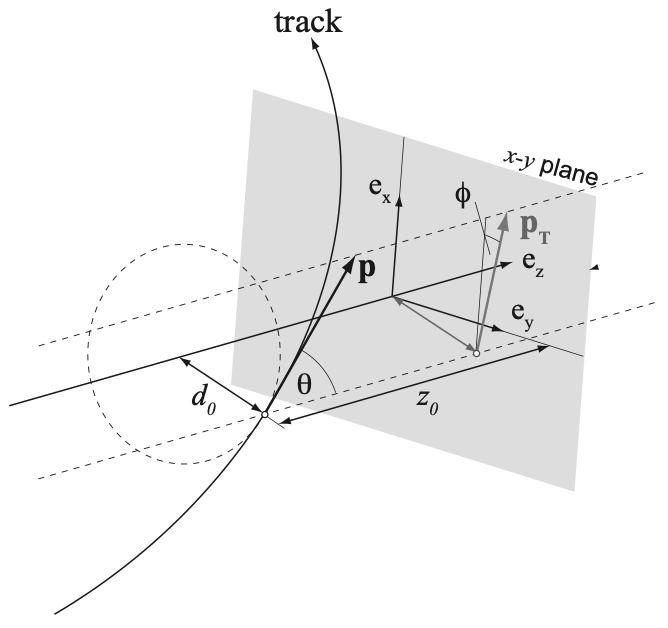
\includegraphics[width=0.6\linewidth]{3_experiment/object_reconstruction/tracking_coordinates.png}
    \caption{Schematic showing the tracking parametrization~\cite{ATLAS-Tracking-2007}.}
    \label{fig:objects:track_vtx:track_parameters}
\end{figure}

The track reconstrucion used in Run-2 uses two complementary approaches: the \textit{inside-out} approach, and the \textit{outside-in}~\cite{ATLAS-NEWT}. 

The first step in the inside-out track reconstruction is the seed-finding, where three hits in the silicon detector are searched for to seed the track reconstruction. Using these three hits and assuming an uniform magnetic field, a first estimate of the track parameters is obtained. Using the track seeds, the track is extrapolated to the other silicon layers, from which a combinatorial Kalman filter is used to estimate the track parameters. At this stage of the process there can be several track candidates for each track seed. Once the track is formed, an ambiguity resolution algorithm is applied to reassign shared clusters to the track with a better match~\cite{ATLAS-NNClustering}, and the final track candidate is fitted using a global \chisq method. The last part of the inside-out method consists on extending the tracks to the \ac{TRT}, and including the \ac{TRT} hits to the track, to improve the track's momentum resolution.

To improve the efficiency for tracks from decays displaced from the original collision point, an outside-in track reconstruction algorithm is also used. The track is seeded with hits from the \ac{TRT}. The track is extended to include hits from the silicon detector, with an ambiguity solver again applied to mitigate the hit sharing between two tracks.

Primary and secondary vertices are of vital importance for the subsequent object reconstruction in \ac{ATLAS}. In this step, the tracks found as explained previously are used as input to the vertexing algorithm~\cite{ATLAS-PVReconstruction,ATLAS-VertexReconstruction}. First of all, the \ac{PV} is defined as the location where two protons collide. \acp{PV} are reconstructed by matching up intersecting tracks, which proceeds in three main steps: seeding, track assignment, and fitting. The vertex with the largest \(\sum \pt^2\) for all associated tracks is labeled as the hard-scatter vertex. There are some particles that decay rapidly after their production, such as \(\tau\) leptons or heavier quarks (\(b\) or \(\cquarks\)), and their decay position can be measured. From the remaining tracks originated from these decays, it is possible to identify secondary vertices. All the remaining reconstructed vertices are considered to be pile-up.








\section{Photons and electrons}

The reconstruction of electrons and photons in \ac{ATLAS} is based on the energy deposition in the \ac{ECAL}. Since electrons and photons leave similar signals in the \ac{ECAL}, their reconstrucion is done simultaneously, distinguishing between them by the reconstructed track information left in the \ac{ID}.


\subsection{Reconstruction}
\label{subsec:objects:egamma:reco}

The \textit{offline} photon and electron reconstruction~\cite{ATLAS-EGamma-Performance-2015-2017,ATLAS-TopoClusters-Run2} makes use of dynamic, variable-size clusters, connected topologically between the \ac{ECAL} and \ac{HCAL} cells~\cite{ATLAS-TopoClusters-Run1}, called topo-clusters. This approach allows for the clusters to recover energy from bremsstrahlung photons or from electrons from photon conversions. With this approach, there are three types of objects:
\begin{itemize}
    \item Electrons: consists of a cluster built from the energy deposits in the \ac{ECAL} and a matched track.
    \item Converted photons: consits of a cluster mathed to a conversion vertex (or vertices)
    \item Unconverted photons: cluster matched to neither an electron track nor a conversion vertex.
\end{itemize}

\begin{figure}[ht!]
    \centering
    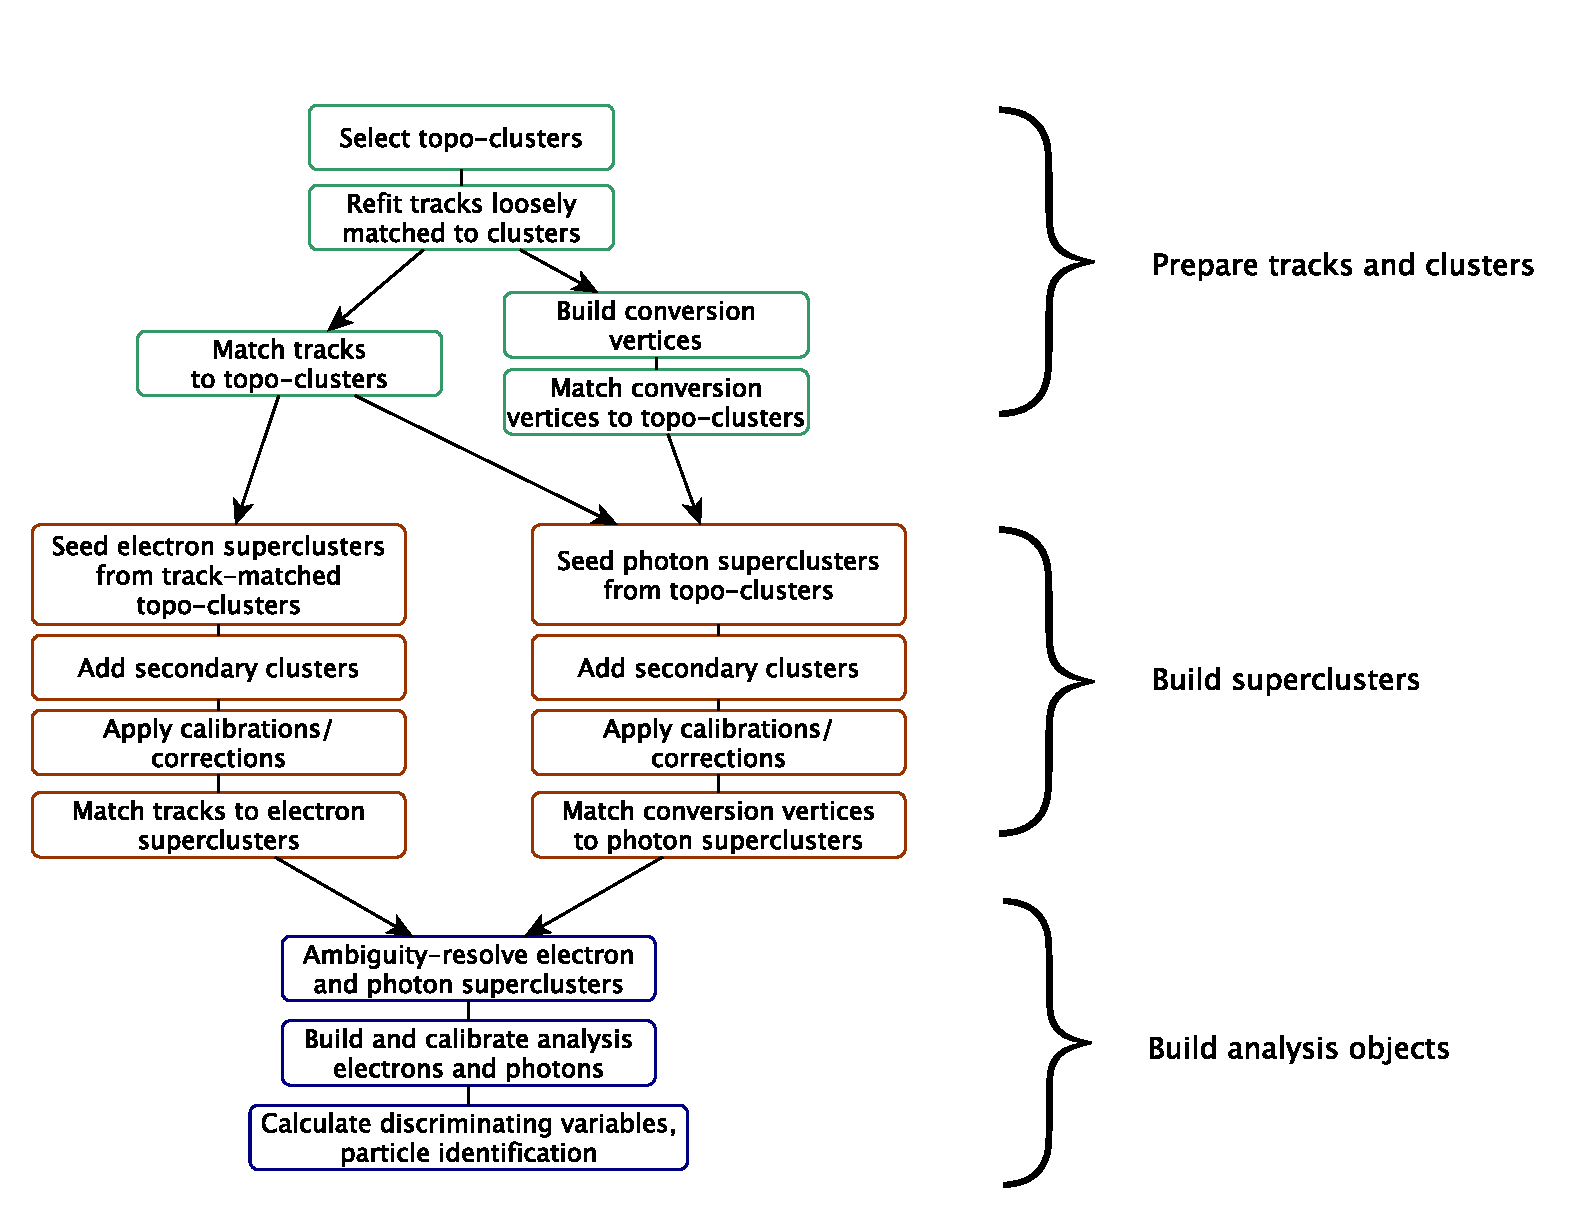
\includegraphics[width=0.8\linewidth]{3_experiment/object_reconstruction/egamma_reconstruction}
    \caption{Diagrama showing the reconstruction algortihm workflow for electrons and photons, extacted from \Refn{\cite{ATLAS-EGamma-Performance-2015-2017}}}
    \label{fig:objects:egamma:reco:reco_diagram}
\end{figure}

The algorithm for the reconstruction of electrons and photons proceeds as shown in \Fig{\ref{fig:objects:egamma:reco:reco_diagram}}.
The reconstruction process begins with the topo-cluster formation. First, proto-clusters are formed in the \ac{ECAL} and \ac{HCAL} by grouping cells that have a required energy, and by subsequently adding neighbouring cells in four consecutive steps, obtaining the topo-cluster. Reconstructions starts only in those cases where the topo-clusters energy in the \ac{ECAL} is greater than \(400~\mev\).

The algorithm also builds conversion vertices out of the refitted tracks and matches them to the selected topo-clusters.
After the initial track-cluster matching and conversion building, the electron and photon supercluster algorithms run separately in parallel. In the first stage, topo-clusters are evaluated for use as seed cluster candidates, which form the basis of superclusters; in the second stage, clusters near the seed candidates are identified as satellite cluster candidates, which may emerge from bremsstrahlung radiation or topo-cluster splitting. Satellite clusters are added to the seed candidates to form the final superclusters, if they pass the necessary selection criteria.
After applying initial position corrections to the resultant superclusters, the reconstruction algorithm matches tracks to
the electron superclusters and conversion vertices to the photon superclusters.

Since one object may be reconstructed as both an electron and a photon, an ambiguity resolution is performed to remove part of the overlap. However, some overlap is allowed in order to maintain a high reconstruction efficiency for electrons and photons, to which physics analyses may apply their own criteria. The final electrons and photons are then built and calibrated, facilitating the calculation of additional variables used for quality cuts and ambiguity resolution



\subsection{Identification}
\label{subsec:objects:egamma:id}

In order to distinguish real photons (those coming from the collision) from background photons which have much larger production cross sections (coming from hadrons decays, also called fake photons), it is necessary to rely on a algorithm of identification with high signal efficiency and background rejection, for photon candidates with \(\pt \sim 10~\gev\) up to the \tev scale. 
Currently, photon identification in ATLAS is based on a set of rectangular cuts on \acp{SSV} computed from the energy deposited in the cells of the cluster in the first and second layer of the \ac{ECAL}, and from the leakage to the \ac{HCAL}. These variables describe the passage of the photons through the calorimeters, characterizing the lateral and longitudinal electromagnetic showers.
The full photon identification process is presented in \Ch{\ref{ch:pid_ss}}, where the \acp{SSV} are explained one by one. Also, \Chs{\ref{ch:ffs}}{\ref{ch:cellrw}} present two approaches to correct the differences seen in these \acp{SSV} between data and \ac{MC}.



\subsubsection{Shower shape variable corrections}

Due to the imperfection of the \ac{ATLAS} simulation to model the \acp{SSV}, and that these variables are used as input to the identification step, it is important that they are corrected. Historically, the corrections are called \acp{FF}, and they comprised modifications to the mean value of the \acp{SSV}, calculated by minimizing the \chisq value between the data and \ac{MC} \acp{SSV}.
More details on the \ac{SSV} corrections are given in GIVE SECTION!!!

Additional corrections to all the reconstructed and identified photons in the simulation are applied event-by-event in the form of scale factors. These values, provided centrally by the \textsc{EGamma} group to \ac{ATLAS}, represent the residual differences on the efficiencies between actual data and \ac{MC}, computed as a function of the photon \pt and pseudo-rapidity \(\eta\) and separately for converted and unconverted photons.








\subsection{Isolation}
\label{subsec:objects:egamma:iso}

To further reduce the backgrounds of jets misidentified as photons and of hadron decay within the jets (such as the case of neutral pions), two isolation variables are defined: \etconefo and \ptconetw.

\begin{figure}[ht!]
    \centering
    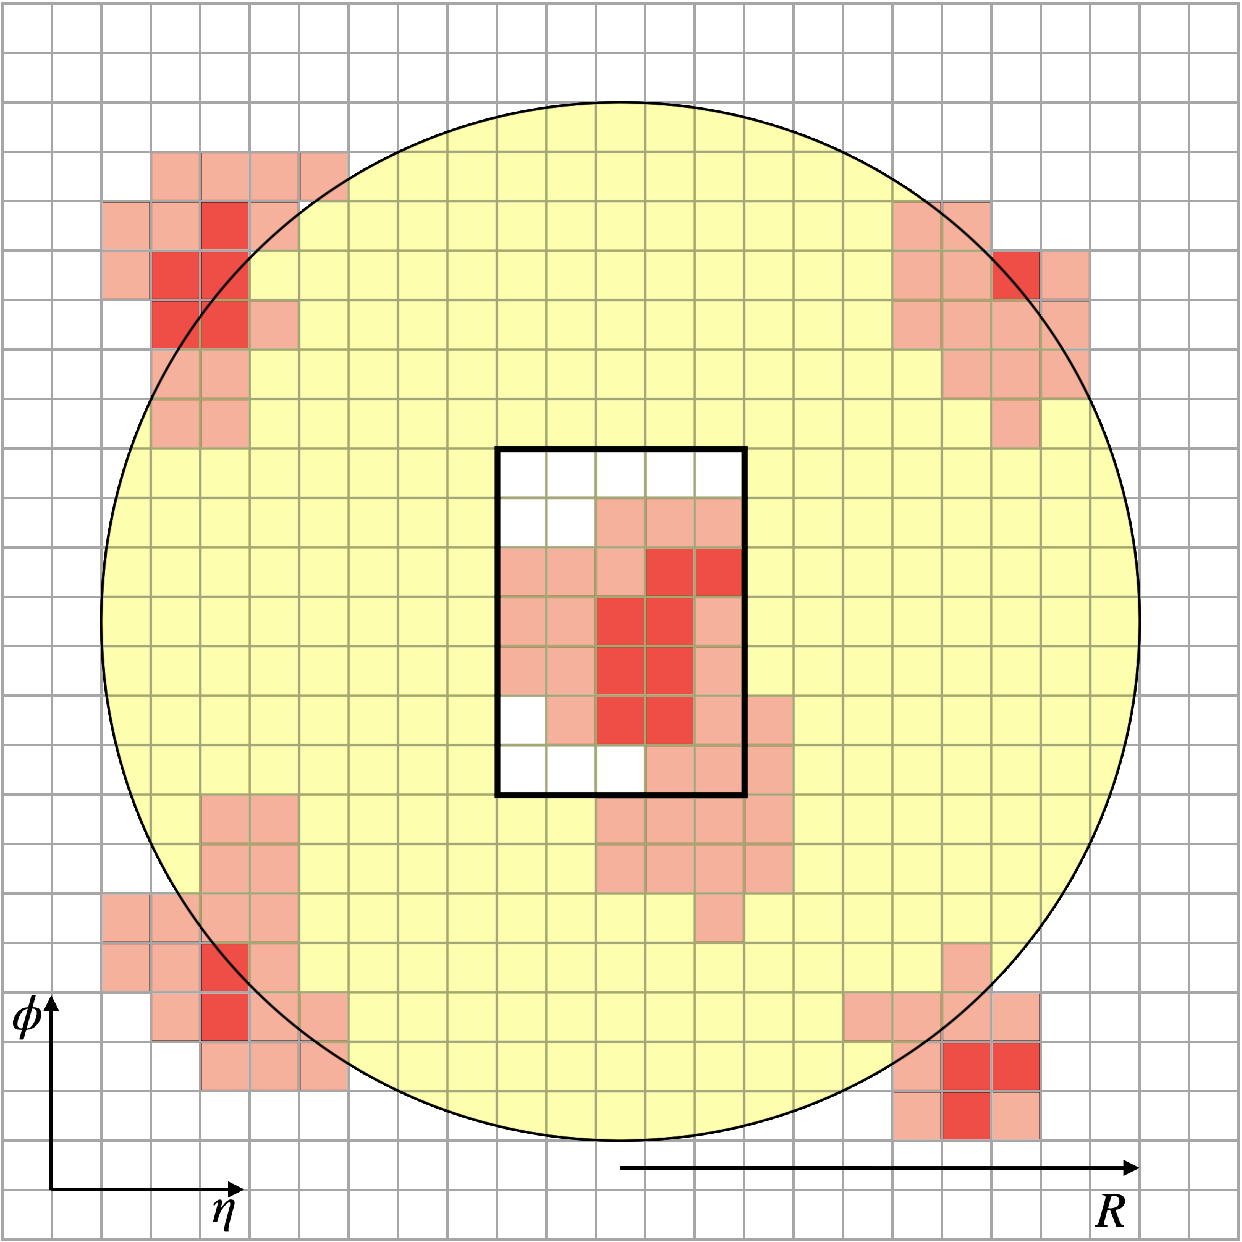
\includegraphics[width=0.5\linewidth]{3_experiment/object_reconstruction/isolation_diagram}
    \caption{Diagram showing the calculation of the calorimetric isolation variable. When \(R=0.4\), \etconefo is computed.}
    \label{fig:objects:egamma:iso:iso_diagram}
\end{figure}

The procedure to compute the isolation energy \etconefo is as follows, and showed in \Fig{\ref{fig:objects:egamma:iso:iso_diagram}}. First, a cone of radius \(\DeltaR<0.4\) is built around the photon or electron candidate, and the energies of all the cells in the topo-clusters (introduced in \Sect{\ref{subsec:objects:egamma:reco}}) whose bary-centers are located inside the cone, are added together. Then, to this computed energy, the energy of all the cells in a \(5\times 7\) window (in units of \(\eta \times \phi\) in the second layer of the \ac{ECAL}) centered around the candidate are subtracted, in order to remove the energy of the candidate itself. Pile-up contributions and energy leakages outside the cone are also taken into account.

The track isolation variable \ptconetw is obtained by adding the \pt of the good-quality tracks in a cone of radius \(\DeltaR<0.2\) around the electron candidate or in the direction of the converted photon cluster.
The track associated to the track or to the converted photon are excluded from this computation, as well as those tracks which do not pass the \textit{good-quality} track requirement. A \textit{good-quality} track is defined as one in which the \pt is \(\pt>1~\gev\), and it has a minimum distance to the primary vertex along the \(z\)-axis of \(|z_0 \sin \theta| < 3\) mm.

In general, for photons and electrons, there is no other energy deposited in the cone around the candidate, apart from the low-energy objects originating from the remnants of the collision, multiple interactions and pile-up. On the other hand, for fake photon candidates and non-direct photons, additional energy is observed within the cone, originating from objects accompanying the jet.

\begin{table}[ht!]
    \caption{Summary of electron and photon isolation \acp{WP} use throughout this thesis.}
    \resizebox{\linewidth}{!}{%
        \begin{tabular}{|l|c|c|c|}
            \hline
            Object                      & WP                             & Calorimetric Isolation                                    & Track Isolation   \\ \hline
            \multirow{3}{*}{Photon}     & \texttt{FixedCutLoose}         & \(E_{T}^{\text{cone20}}<0.065\times \pt \)                & -                                  \\
                                        & \texttt{FixedCutTightCaloOnly} & \(\etconefo < 0.022\times \pt + 2.45~\gev\)               & -                                  \\
                                        & \texttt{FixedCutTight}         & \(\etconefo < 0.022\times \pt + 2.45~\gev\)               & \(\ptconetw/\pt < 0.05\)           \\ \hline
            \multirow{2}{*}{Electron}   & \texttt{Loose\_VarRad}         & \(\etconetw < 0.2\times\pt\)                              & \(\pt^{\text{cone30}}/\pt < 0.15\) \\
                                        & \texttt{HighPtCaloOnly}        & \(\etconetw < \max\left(0.015\times\pt, 3.5~\gev\right)\) & -                                  \\ \hline
        \end{tabular}
    }
    \label{fig:objects:egamma:iso:iso_table}
\end{table}

From the calorimetric and track isolation different \acp{WP} can be defined separately for both electrons and photons. For electrons, two strategies are defined: either to achieve a fixed effiicency, or to apply fixed cuts on the isolation variables. In the case of photons, there are \acp{WP} which do not use both the isolation variable, as is the case of the \texttt{FixedCutTightCaloOnly} \ac{WP}, which only uses calorimetric isolation. The definitions of the different \acp{WP} used throughout this thesis is shown in \Tab{\ref{fig:objects:egamma:iso:iso_table}}. Also, it is common to define the following variables for the photon \texttt{FixedCutTight} \ac{WP}:
\begin{align}
    \etiso &= \etconefo - 0.022 \times \et - 2.45~\gev\\
    \ptiso &= \ptconetw / \et
\end{align}
therefore leaving the \texttt{FixedCutTight} \ac{WP} defined as
\begin{align}
    \etiso &< 0 ~\gev\\
    \ptiso &< 0.05 
\end{align}















\section{Muons}



The rate of bremsstrahlung radiation is inversely proportional to the square of a particle's mass. Since muons are about 200 times heavier than electrons, they primarily interact with the detector material through ionization. Therefore, muons are minimally ionizing particles that do not create electromagnetic shower in the calorimeters and pass through all layers of the \ac{ATLAS} detector. Hence, muon detection relies on track measurements from the \ac{ID} and \ac{MS}. The combination of the two subdetectors define four types of muons, depending on the used information for the reconstruction:
\begin{itemize}
    \item \acp{CB}: muons reconstructed from a global refit of \ac{ID} and \ac{MS} tracks
    \item \acp{ST}: muons reconstructed from a fitted \ac{ID} track and \ac{MS} segment track
    \item \acp{CT}: muons reconstructed using \ac{ID} track matched to the minimum ionizing energy deposits in the calorimeters
    \item \acp{ME}: muons reconstructed solely from \ac{MS} tracks.
\end{itemize}


The overlap between different types of muons is resolved as follows. When two muon types share the same \ac{ID} track, the order of preference is: first \ac{CB}, then \ac{ST} and finally \acp{CT}. The overlap with \acp{ME} is solved by analyzing the hits of the tracks, selecting those tracks with the best fit and the highest number of hits.

For the muon identification, quality cuts are applied to distinguish isolated muons from those coming from background processes, mainly from pion and kaon decay.
The variables with good discriminating power used are described in \Refn{\cite{ATLAS-Muon-Performance-2016}}. Four identification selections are defined: Loose, Medium, Tight, and High-\pt. The first three categories are inclusive, and Medium being the default selection in \ac{ATLAS}. Finally, the muon candidates to be used by the analyses are asked to satisfy the isolation requirements, both at traack and calorimetric levels, analogously to what was detailed for photons in the previous section. For the first case, a variable similar to that used for photons is used, but with a variable-radius cone \(\DeltaR = \min(10~\gev/\pt, 0.3)\) around the muon \pt, excluding the muon track. For calorimetric isolation the same variable \etconefo is used, with the difference of using a radius of \(R=0.2\), instead of \(0.4\) as before. Based on these variables, 7 isolation selection criteria (7 \acp{WP}), optimized for different analyses, are defined.








\section{Jets}


Due to color confinement in \ac{QCD}, a quark or gluon cannot exist on its own and goes through hadronization to form a collimated color-neutral stream of particles, \textit{jets}. Generally, jets penetrate through the \ac{ECAL} and get fully absorbed by the material in the hadronic calorimeter. In the following, a brief description of the typical clustering method adopted by \ac{ATLAS} is given. Also, the two existing types jet reconstruction are described.


\subsection{\Antikt jet clustering algorithm}

Given that jets are constituted by a high number of particles that leave energy depositiions in the \ac{ECAL} and \ac{HCAL} and tracks in the \ac{ID}, a clustering algorithm groups together constituents in the event to define the jets. Said algorithm is called the \antikt algorithm~\cite{AntiKtAlgorithm}. In the same way as for electrons and photons, \ac{ATLAS} jet reconstruction relies on the formation of \topos: grouped energy depositions in the calorimeters cells using a sequential combination algorithm. Then, the \antikt algorithm combines the \topos with the following steps:
\begin{itemize}
    \item Measure the distance between all \topos between themselves, and of each \topo with the beam:
        \begin{gather}
            \dij = \min \left( p_{T,i}^{-2}, p_{T,j}^{-2} \right) \frac{\Delta_{i,j}^2}{R^2}\\
            d_{iB} = p_{T,i}^{-2}
        \end{gather}
        where \(\Delta_{ij}^2 = \Delta\phi_{ij}^2 + \Delta\eta_{ij}^2\) and \(R\) is the jet-radius.
    \item If the minimum of all the distances computed previouly is \(d_{iB}\), the \topo \(i\) is classified as a jet, and is discarded in successive iterations.
    \item If the minimum of all the distances is \(d_{ij}\), \topos \(i\) and \(j\) are combined, all the distances are computed again with this new \topo and the iteration is carried all over again.
\end{itemize}
This process is repeated until all te particles in the event have been clustered.

The \antikt algorithm starts by clustering the radiation around the hardest particle in the event since the leading \pt particle will define the \(\min \left( \frac{1}{p_{T,i}^2}, \frac{1}{p_{T,j}^2}  \right)\) term in the \dij definition. This allows jets in the event to have a stable direction early on the combination process. The \antikt algorithm is preferred to other sequential jet algorithms since jets have regular boundaries which are approximately conical, shown in \Fig{\ref{fig:objects:jets:antikt}}. Jets originating from quarks or gluons in general are called small-\(R\) jets and a radius of \(R=0.4\) is used for their reconstruction. On the other hand, jets representing massive particles which decay hadronically are called large-\(R\) jets, and use \(R=1.0\). The usage of a wider cone helps to include the majority of the particles product of the decay.


\begin{figure}[ht!]
    \centering
    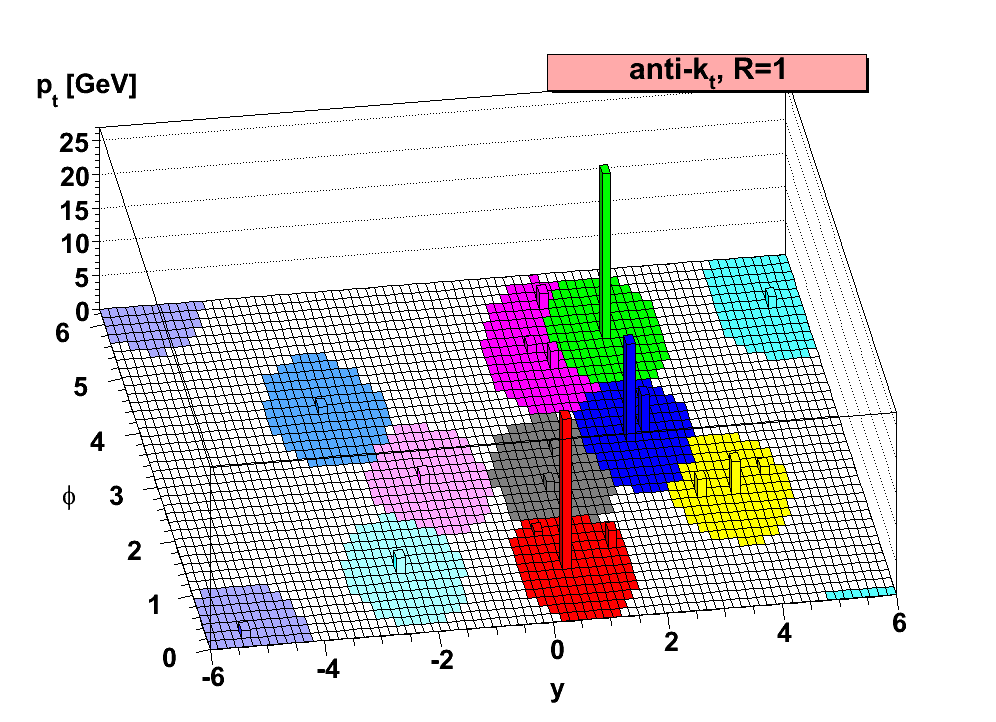
\includegraphics[width=0.7\linewidth]{3_experiment/object_reconstruction/antikt_clusters}
    \caption{Schematic representation of the \antikt algorithm for jet clustering~\cite{AntiKtAlgorithm}.}
    \label{fig:objects:jets:antikt}
\end{figure}

\subsection{Calorimeter Jets}

One way to reconstruct jets is based on energy deposits in the calorimeter. In a similar way to what has been explained for electrons and photons in \Sect{\ref{subsec:objects:egamma:reco}}, energy depositions on the cells of the \ac{ECAL} and \ac{HCAL} are used to build \topos, which approximates the energy deposits of individual hadrons~\cite{ATLAS-TopoClusters-Run1,ATLAS-TopoClusters-Run2}. Jets reconstructed in this manner and clustered with the \antikt algorithm with a radius of \(R=0.4\) are referred as \textsc{EMTopo} jets, and are the proxies for the individual quarks and gluons. In the jet reconstruction, only the \topos with positive net energy are included.

\subsection{PFlow Jets}

Another approach for jet reconstruction is taken in the particle flow algorithm, in which measurements from both the tracker and the calorimeter are combined to form the signals, which ideally represent individual particles.
In this alorithm, tracks are matched to \topos using proximity in \((\eta,\phi)\) space, also accounting for the size of the \topo. The tracks are only “matched” if the cluster carries more than \(10\%\) of the track's momentum. Sometimes the \topo fails to cluster all of the hadron's energy in a single \topo. In cases where the expected energy of the track is less than the expected track's energy, a “split shower recovery” combines nearby \topos to form a \topo set. From this \topo set, the expected energy of the track is subtracted from the \topo's cells, starting with high-energy density cells. If the residual energy is consistent with the resolution of the expected track energy, the residual energy is also subtracted in the last step called “remnant removal”.

The result of this algorithm is a set of tracks, modified and unmodified \topos which are the \ac{PFlow} objects. The \ac{PFlow} objects can also be clustered with the \antikt algorithm and the same \(R=0.4\) to form \ac{PFlow} jets.

There quite a lot of benefits of using the \ac{PFlow} algorithm over the \textsc{EMTopo} one:
\begin{itemize}
    \item The momentum resolution of the tracker is significantly better than the calorimeter's energy resolution for low-energy charged particles.
    \item Allows for a higher acceptance for softer particles. Tracks are reconstructed for charged particles with a minimum \pt of \(400~\mev\), and oftentimes these particles' energy deposits do not pass the thresholds to seed \topos.
    \item Improved angular resolution of a single charged particle as it uses the tracker information instead of the calorimeter's.
    \item Low-\pt charged particles originating within a hadronic jet are swept out of the jet cone by the magnetic field by the time they reach the calorimeter. By using the tracks azimuthal coordinate at the perigee, these particles are clustered into the jet.
    \item It is possible to remove those tracks originating from pile-up, knowing that these do not originate from the \ac{PV}.
\end{itemize}

However, particle flow introduces a complication. For any particle whose track measurement ought to be used, it is necessary to correctly identify and subtract its signal in the calorimeter to avoid double-counting. In the particle flow algorithm, a boolean decision is made as to whether to use the tracker or calorimeter measurement. The ability to accurately subtract all of a single particle energy, without removing energy deposited by other particles, forms the key performance criterion upon which the algorithm is optimised.

In this thesis, \ac{PFlow} jets are considered, as they have proven to provide better jet reconstruction~\cite{ATLAS-JetPFlow-Performance}, principally for those with low \pt and in the \met reconstruction~\cite{ATLAS-MET-Performance-2016}.


\subsection{Jet calibration}

Once the jets are reconstructed, their 4-momentum is corrected to match the kinematics of a truth jet\footnote{The truth jets come from the \antikt clustering of the stable final state truth particles (hadrons and charged leptons) in simulation.}, as shown in \Fig{\ref{fig:objects:jets:jet_calib:jet_calib_sequence}}. The first three corrections account for contamination from the underlying pile-up distribution and fluctuations due to the origin of the jet~\cite{ATLAS-Jet-Calibration-Run2}. The Global Sequential Calibration improves the jets \pt resolution (and associated uncertainties) by sequentially removing the dependence of the reconstructed jet response (\(R= E^{\text{reco}} / E^{\text{truth}}\)) on key event observables. Finally, the residual differences between data and \ac{MC} are accounted for by
measuring the momentum imbalance in \Zjets, \gammajet and multi-jet events.

\begin{figure}[ht!]
    \centering
    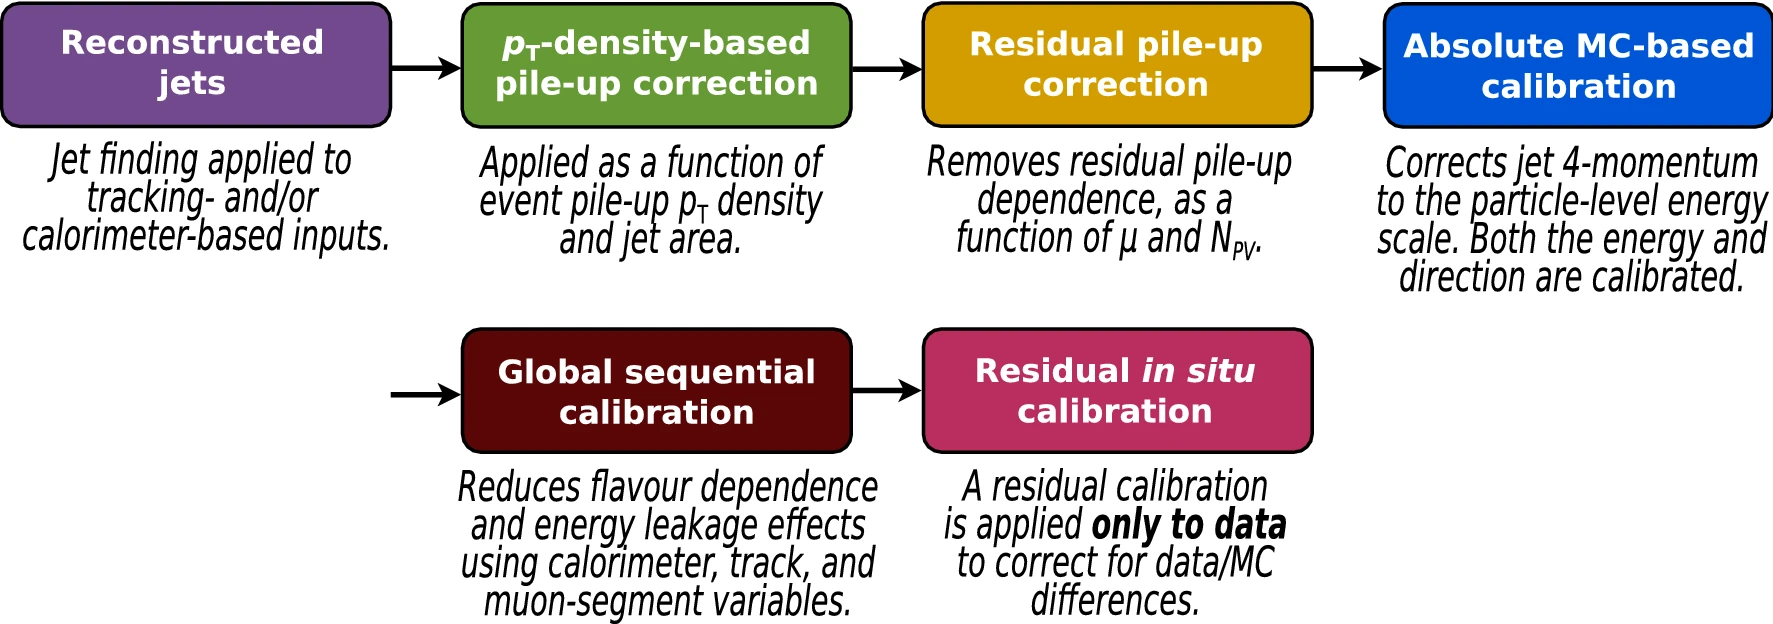
\includegraphics[width=\linewidth]{3_experiment/object_reconstruction/jet_calibration}
    \caption{\texttt{PFLow} 4-momemtum jet calibration steps~\cite{ATLAS-Jet-Calibration-Run2}.}
    \label{fig:objects:jets:jet_calib:jet_calib_sequence}
\end{figure}

To reduce the number of jets with a considerable fraction of energy coming from pile-up, the \ac{JVT} algorithm is used. This algorithm \fixme{update to NNJVT} reconstructs a multivariate discriminant that combines, among other quantities, the \ac{JVF} (fraction of the tracks' \pt associated to a jet originating from the \ac{PV}, and the total number of tracks) and the number of \acp{PV} in the event \Npv. As the jets that do not originate from the hard-scatter interaction are generally softer, the \ac{JVT} cut is applied only to jets with \(\pt<60~\gev\) and \(\abseta<2.4\). The default \ac{JVT} \ac{WP} is \(96\%\) efficient for hard-scatter jets.
















\section{Jet flavor tagging}

Heavy hadrons decays are governed mainly by the heaviest hadron in the decay cascade. A \(b\)-hadron generally decays through a cascade to a \(c\)-hadron, which in turn decays to an \(s\)-hadron, etc, which leads to the existence of multiple vertices.

\ac{FTAG} is the classification of jets containing \(b\)-hadrons (\bjets), \(c\)-hadrons (\cjets) or neither \(b\)-
or c-hadrons (light-flavour jets, or \ljets) by using algorithms sensitive to the distinctive properties of the respective classes.
These complex algorithms rely on the multiple vertices, on the high mass, high decay multiplicity and characteristic decay modes of the \(b\)- and \(c\)-hadrons, as well as on the properties of heavy-quark fragmentation.


In \ac{ATLAS} a two-step approach is employed to reconstruct key characteristics of heavy-flavour jets. In the first stage, low-level algorithms use complementary methods to extract track information from the charged particles linked to the jet. Some algorithms focus on the properties of individual tracks, while others analyse their correlations or combine them to explicitly reconstruct displaced vertices. In the second stage, the outputs from these algorithms are integrated into a high-level algorithm using multivariate classifiers to optimize performance. Over time, the algorithms have evolved significantly, starting with likelihood-based discriminants and boosted decision trees during \ac{LHC} Run-1, and progressing to more advanced methods like recurrent and deep neural networks, resulting in notable improvements on the identification performance~\cite{ATLAS-FTAG-Calibration-2012,ATLAS-FTAG-Efficiency-2012,MV2Algorithm,ATLAS-FTAG-DeepLearning}.

Starting in Run-3, a novel Transformer-based "GN2" algorithm is developed by the \ac{FTAG} combined performance group in \ac{ATLAS}. The GN2 algorithm is a single trained model which supersedes DL1d~\cite{ATLAS-FTAG-DL1-Run2} and the low level algorithms that feed it. It is based on GN1~\cite{ATLAS-FTAG-GN1}, and was quickly refied into GN2. GN2 replaces the Graph Attention Network~\cite{GANs} used by GN1 with a Transformer~\cite{GN2Transformer}, and also benefits from several other architectural optimisations and from an order of magnitude more training statistics.

GN2 directly accepts information about the jet and associated tracks and as such does not depend on other flavour tagging algorithms. GN2 retains the two the auxiliary training objectives that were introduced with GN1: the grouping of tracks originating from a common vertex, and the prediction of the underlying physics process from which each track originated.

This new algorithm is also prepared to provide identification of \cjets and jets originating from \(\tau\) decays. Outputs of this tagger comprise the probabilities of a jet to be tagged as a \(b\)-, \(c\)-, \(\tau\)- and light-flavor jet, labeled as \(p_b\), \(p_c\), \(p_{\tau}\) and \(p_u\), respectively.

\subsection{\bjet identification performance}

In order to evaluate the performance of the tagger of identifying \bjets at a constant efficiency, the ability to reject \(c\)-, \(\tau\)- and light-flavor jets is measured. The tagger output probabilities are combined to build a single discriminant \gntb, defined as
\begin{equation}
    \gntb = \log \left(
        \frac{p_b}{f_c p_c + f_{\tau} p_{\tau} + \left(1-f_c-f_{\tau}p_u\right)}
    \right).
\end{equation}
The parameters \(f_{c(\tau)}\) are free and determine the weighting between \(p_{c(\tau)}\) and \(p_u\) in the discriminant. The specific values of these parameters are determined through an optimisation procedure aimed at maximimsing the rejection of \cjets (\(\tau\)-jets) and \ljets and found to be \(0.2\) (\(0.01\)).


From the tagger discriminant score, several \acp{WP} can be defined, simply by requiring the \gntb score to by above a certain threshold. The \ac{FTAG} working group provides centrally to the whole \ac{ATLAS} collaboration 5 different \acp{WP} to achieve a fixed overall \btagging efficiency: \(65, 70, 77, 85\) and \(90\%\) efficiency, and are shown in \Fig{\ref{fig:objects:jet_tagging:btag_discrminant}}. In said figure, the data and \ac{MC} GN2 tagger distributions are compared, where the different flavour contributions are shown with different colors.

\begin{figure}[ht!]
    \centering
    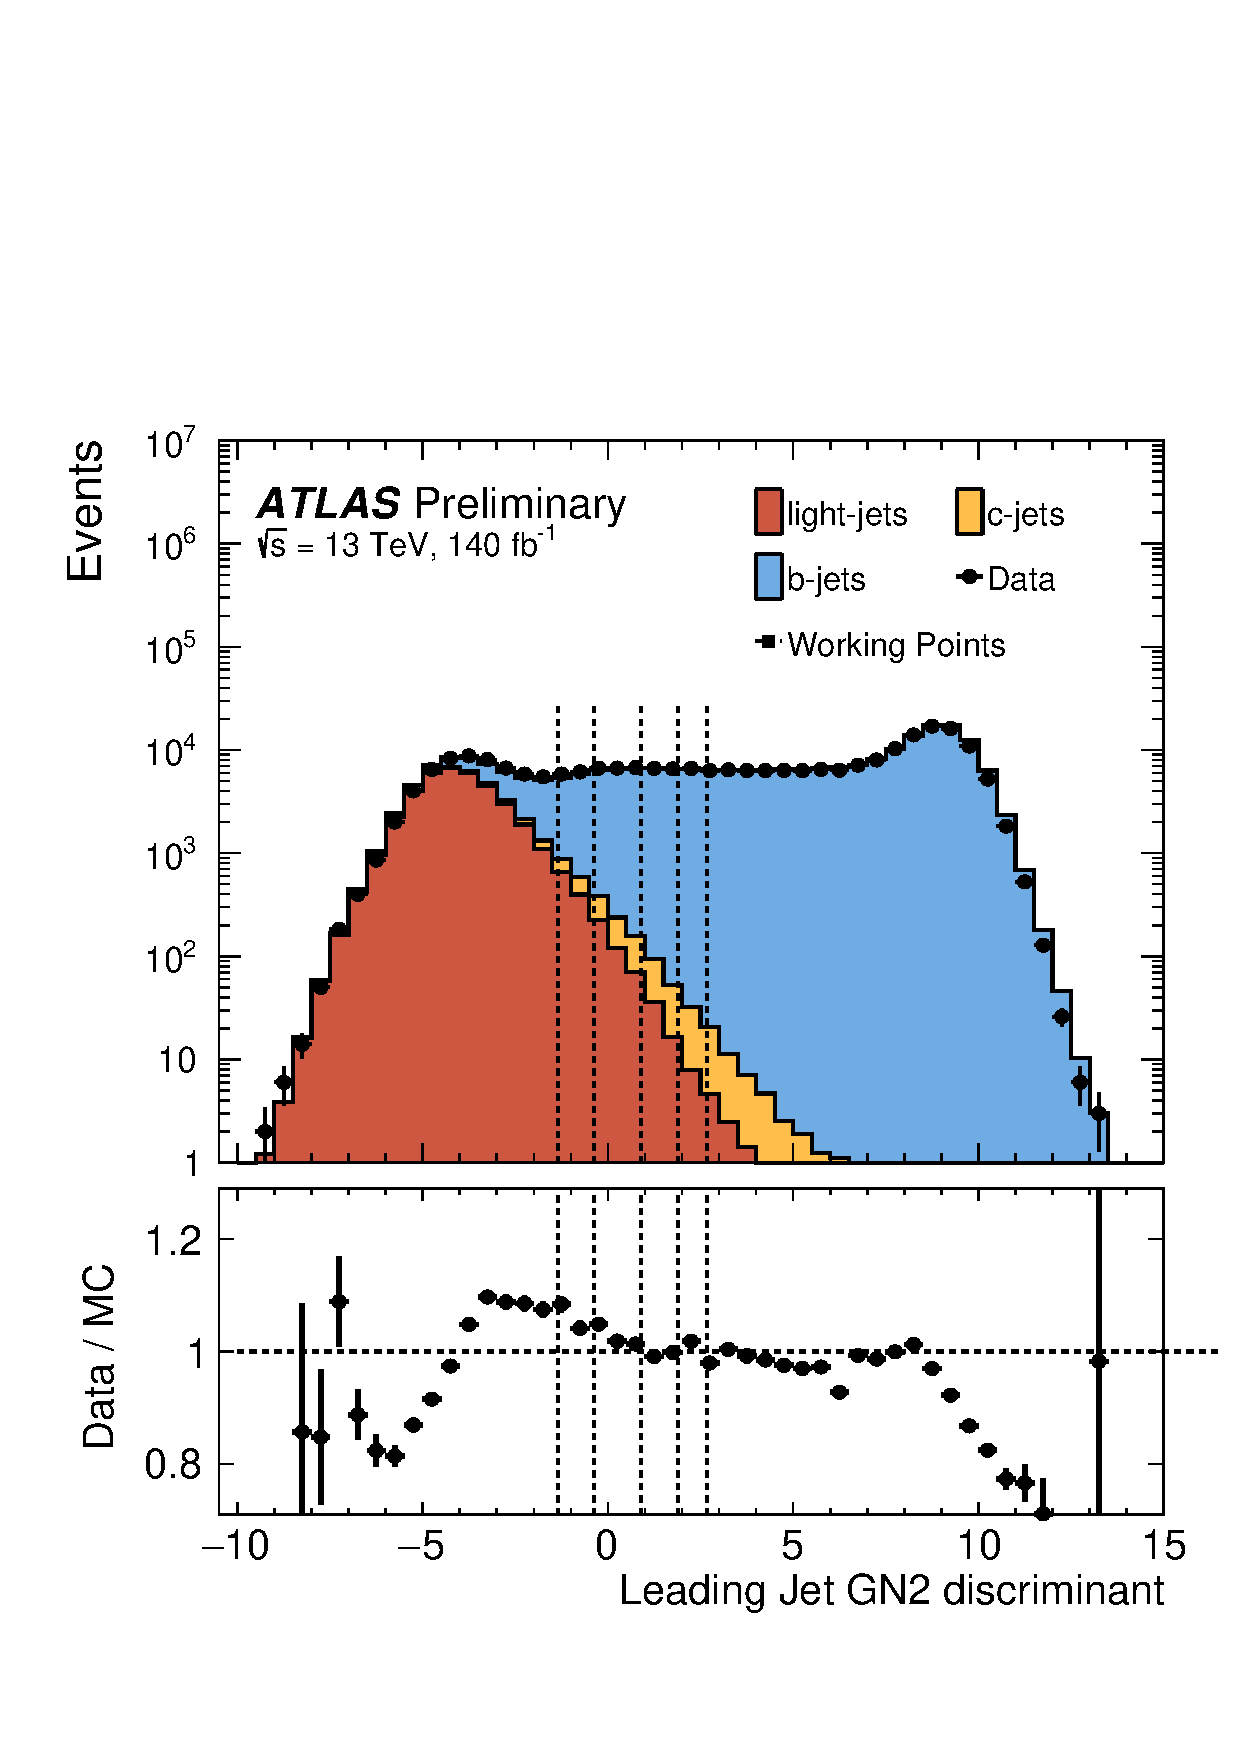
\includegraphics[width=0.6\linewidth]{3_experiment/object_reconstruction/btagging_discriminant}
    \caption{GN2 tagger discriminant comparison between data and single-lepton \ttbar \ac{MC} simulation. The \(l\)-, \(b\)- and \cjets are contributions are shown with different colors, and the 5 \btag \acp{WP} shown with the dashed vertical lines. From left to right, the dashed lines represent the \(90, 85, 77, 70\) and \(65\%\) efficiency \acp{WP}. The lower pad shows the ratio between data and the stacked \ac{MC}~\cite{ATLAS-FTAG-GN2BtagWPs}.}
    \label{fig:objects:jet_tagging:btag_discrminant}
\end{figure}

One key challenge of \btagging is the decrease in efficiency at higher \pt. In this high-\pt regime, particles become more collimated and they tend to travel further in the \ac{ID} before decaying, potentially leading to a decay track with spurious hits. The degraded efficiency is visualised in \Tab{\ref{tab:objects:ftag:btag_efficiency_original}}, where tagging efficiencies are shown for \bjets, along with \cjets, \ljets and \tjets rejections, in the low and high-\pt regimes. The values shown are computed by using different samples, where \ttbar is used at low-\pt and \(Z'\) decay events~\footnote{The leptophobic axial-vector \(Z'\) model is a simplified Dark-Matter model in which one of the theorised decay products are a pair of quarks.} are used in the high-\pt region. It can be seen that the \btag efficiency drops by \(30\%\) for higher \pt jets.

\begin{table}[ht!]
    \caption{Measured \btagging efficiencies and \cjets, \ljets and \tjets rejections in the low and high-\pt regime.}
    \label{tab:objects:ftag:btag_efficiency_original}
    \begin{tabular}{llcccc}
    \toprule
    Sample & \pt range [\gev]                                    & $b$-efficiency & $c$-rejection & light-flavor rejection & $\tau$-rejection \\ \midrule
    $t\bar{t}$  & \(20<\pt<250\)    & $0.76$         & $17.52$       & $448.61$               & $71.15$          \\
    $Z'$        & \(250<\pt<6000\)  & $0.41$         & $20.27$       & $179.99$               & $452.94$         \\ \bottomrule
    \end{tabular}
\end{table}

\subsection{\cjet identification performance}

Similar to \btagging, a single discriminant can be built from the output probabilities of the tagger in order to identify \cjets against \bjets, \(\tau\)-jets and \ljets:
\begin{equation}
    \gntc = \log \left(
        \frac{p_c}{f_b p_b + f_{\tau} p_{\tau} + \left(1-f_b-f_{\tau}p_u\right)}
    \right)
\end{equation}
where now the \(f_{b(\tau)}\) are the free parameters that control the rejection between \(b\)-, \(\tau\)- and light-flavor jets. Using the same optimisation procedure as for \btagging, the values for \(f_{b(\tau)}\) are found to be \(0.3\) (\(0.05\)).

Thanks to the great \btagging efficiency achieved by GN2, it is possible to design a \ctagging \ac{WP} after applying \btagging-veto, further separating \cjets from \ljets. By building this simultaneous tagging \ac{WP} and assuming the fraction of \tjets to be negligible, one can separate light-, \(c\)- and \(\bjets\) in three orthogonal regions. Starting from requiring a jet to \textit{not} pass the \(77\%\) \btagging \ac{WP} (\btag veto), three different \ctagging \acp{WP} are defined by fixing the \gntc score: \(10, \, 30\) and \(50\%\) \ctag efficiency. The efficiency and rejection measurements for the both samples described above, after applying the \(50\%\) \ctag \ac{WP} are shown in \Tab{\ref{tab:objects:ftag:ctag_efficiency_original}}.

\begin{table}[ht!]
    \caption{Measured \ctagging efficiencies and \bjets, \ljets and \tjets rejections in the low and high-\pt regime. The values shown correspond to those after applying the \btagging \(77\%\) \ac{WP} veto and the \(50\%\) \ctagging \ac{WP}. \fixme{rejection values not correct!}}
    \label{tab:objects:ftag:ctag_efficiency_original}
    \begin{tabular}{llcccc}
    \toprule
    Sample & \pt range [\gev]                                    & $c$-efficiency & $b$-rejection & light-flavor rejection & $\tau$-rejection \\ \midrule
    $t\bar{t}$  & \(20<\pt<250\)    & $0.467$         & $17.52$       & $448.61$               & $71.15$          \\
    $Z'$        & \(250<\pt<6000\)  & $0.344$         & $20.27$       & $179.99$               & $452.94$         \\ \bottomrule
    \end{tabular}
\end{table}


\fixme{Add plots with GN2 distributions?}












% \subsection{Monte Carlo generators}

% \paragraph{Sherpa}
% One of the general purpose event generators used in this thesis is \texttt{SHERPA} \cite{Sherpa}.  It includes matrix element generators as well as a built-in parton showering.  In this thesis,  simulated events with \texttt{SHERPA} include Multi-boson processes as well as the associate production of vector bosons and jets.  

% \paragraph{Powheg} 
% The \texttt{POWHEG} \cite{Powheg} framework is a matrix element generator at next-to-leading perturbative order.  The matrix element generation is interfaced with generators like \texttt{PYTHIA} or \texttt{HERWIG++} in order to simulate the parton shower.  This kind of combination of matrix element generator and parton shower simulation is used or top-related processes such as top-antitop pair production. 

% \paragraph{MadGraph5\_ aMC@NLO} \texttt{MadGraph5} \cite{Madgraph} is used as a matrix element calculator at next-to-leading perturbative order.  Similar to \texttt{POWHEG},  it is interfaced with \texttt{PYTHIA} or \texttt{HERWIG} to include parton showering. 

% \paragraph{Pythia}
% A second general purpose event generator used in this thesis is \texttt{PYTHIA 8}\cite{pythia},  even with matrix element calculation and parton showering possible within \texttt{PYTHIA}, it is widely used for its parton showering,  interfaced with \texttt{POWHEG} or \texttt{HERWIG}.  Additionally,  \texttt{PYTHIA} is used in this thesis to simulate minimum-bias proton-proton collisions.

% \paragraph{Herwig} The \texttt{HERWIG} \cite{Herwig,Herwig++} Monte Carlo event generator has capabilities to be used to simulate the matrix element,  but is only used within this thesis as a variation of the \texttt{PYTHIA} parton showering. 

% \paragraph{EvtGen}
% \texttt{EvtGen} \cite{EvtGen} is a framework that simulates the decay of final state particles.  Events associated with the production and decay of a top quark used in this thesis are simulated through a combination of \texttt{POWHEG}, \texttt{PYTHIA} and \texttt{EvtGen}.  Within this thesis, all events generated with a parton showering by \texttt{PYTHIA} include final state particle decays simulated with \texttt{EvtGen}.

% \subsection{ATLAS detector simulation}
% \label{sec:DAQ:AF2}


% To directly compare the data collected with the ATLAS detector with the prediction of \ac{SM} and \ac{BSM} events in simulation,  the interaction of the produced particles with the detector material has to be simulated.
% The Geant4 \cite{Geant4} software package is used to simulate the interaction of particles with the detector material.
% A full Geant4 model of the ATLAS detector is used to simulate the transition of particles produced in proton-proton collisions through the different detector layers. 

% The simulation of a large number of interactions necessary to mimick the ATLAS reconstruction is computationally extensive.  Especially the simulation of shower developments in the calorimeters consumes a large amount of CPU and computing time. 
% For many \ac{BSM} searches,  a large number of parameters affecting the predicted particle masses and interactions have to be simulated.  A 'fast' parameterised detector simulation has been developed to cope with this high simulation demand.  A so-called Atlfast-II or AFII setup simulation chain uses Geant4 simulation for the interactions in the \ac{ID} and muon spectrometer,  but a parametrised simulation called FastCaloSim for the particle interactions in the electromagnetic and hadronic calorimeter. 
% The improvements in computing time compared to Geant4 simulation of the full detector as well as a fast,  simplified Geant4 simulation is shown in Figure \ref{fig:DAQ:AFIIvsG4}.  The overall processing time is reduces by roughly an order of magnitude compared to the full Geant4 simulation \cite{AFIIprinciple}. 
% \begin{figure}[h]
% \centering
% \includegraphics[width=0.8\linewidth]{figures/DAQ/AFII_CPU_improvement.png}
% \caption{CPU time distributions for 250 $ \ttbar $ events compared for G4,  fast G4 and AFII setup,  taken from \cite{AFIIprinciple} \label{fig:DAQ:AFIIvsG4}}
% \end{figure}
% The fast calorimeter simulation FastCaloSim uses a parametrisation of the calorimeter response.  The parametrisation has been extracted through Geant4 simulation and tunes to data. 
% The main three simplifications include simplifying the detector geometry,  approximating the calorimeter cells as cuboids,  only reproducing the average lateral energy distributions and restricting the simulation to three types of initial particles. 

